\documentclass[titlepage,11pt]{article}

\textwidth 6.5in
\textheight 9in
\oddsidemargin -0.2in
\topmargin -0.5in

\usepackage{indentfirst,graphics,alltt,epsfig,color}

\title{iBioSim Tutorial}

\author{Chris J. Myers}

% \date{Created: August 11th, 2008\\
%   Last Revised: February 3rd, 2010
% }

\begin{document}

\maketitle

%show only subsection granularity in the toc
%\setcounter{tocdepth}{2} 
  
\tableofcontents

\clearpage
  
%\setlength{\parindent}{0em}
%\setlength{\parskip}{10pt}

\section{Introduction}

\noindent
{\tt iBioSim} has been developed for the modeling, analysis, and design of genetic circuits.  While the primary target of {\tt iBioSim} is models of genetic circuits, models representing metabolic networks, cell-signaling pathways, and other biological and chemical systems can also be analyzed.  {\tt iBioSim} includes the following components: 

\begin{itemize}
\item Model Editor - a tool to create a model of a genetic circuit or other biological system.
\item LPN Model Editor - a tool to create a model using a \emph{labeled Petri net} (LPN).
\item Analysis Tool - an abstraction-based ODE, Monte Carlo, and Markov analysis tool.
\item TSD Graph Editor- a tool to visualize TSD files. 
\item Histogram Graph Editor - a tool to visualize probability data. 
\end{itemize}

This tutorial illustrates each of these features of {\tt iBioSim} using a simple model for the \emph{cI} and \emph{cII} genes and the $P_R$ and $P_{RE}$ promoters from the phage $\lambda$ decision circuit.  

% TODO: add figures and more description of the example

\section{Project Management}

\noindent
Within {\tt iBioSim}, all files are collected within projects.   A project is a collection of models, analysis views, learn views, and graphs.  As shown below, {\tt iBioSim} displays all project files on the left, the open models, views, and graphs on the right, and a log of all external commands on the bottom.  The menu bar is located on the top of the window in the Windows and Linux versions.  It is located on the top of the screen in the MacOS version.

\begin{center}

\includegraphics[height=90mm]{screenshots/iBioSim}
\end{center}

\noindent
To create a new project, select New $\rightarrow$ Project from the File menu as shown below.  You will then be prompted to browse to a desired location and to give a name to the project directory.  Enter the name {\tt Tutorial}.  After you do this, click the new button and a new project directory will be created.  

\begin{center}
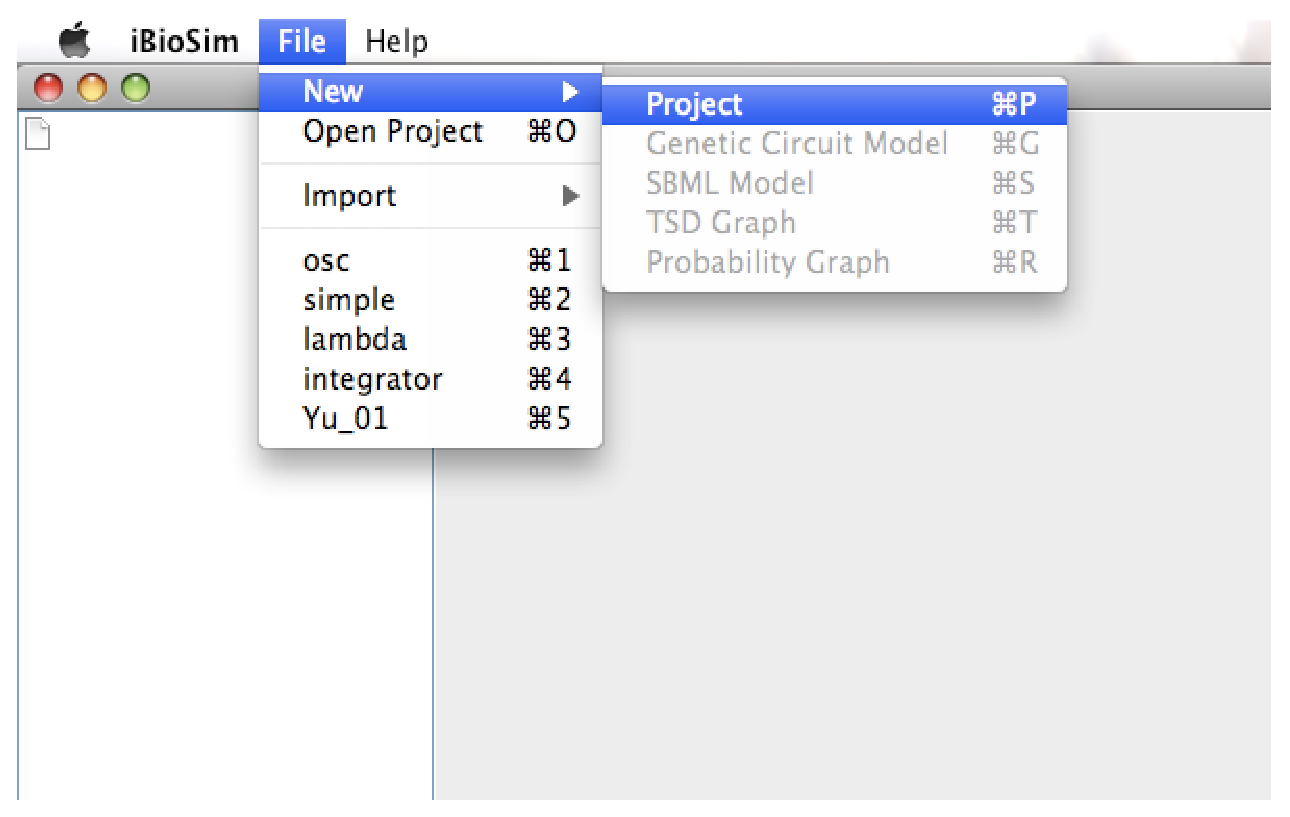
\includegraphics[height=80mm]{screenshots/project}
\end{center}

\section{Model Editor}

\noindent
After you have created a project, you can create a new model to add to the project by selecting New $\rightarrow$ Model from the File menu as shown below. You will then be prompted to enter a model id.  Enter {\tt lambda} (do not select ``Make Grid'' at this time).  At this point, a Model editor will open in a new tab.

\begin{center}
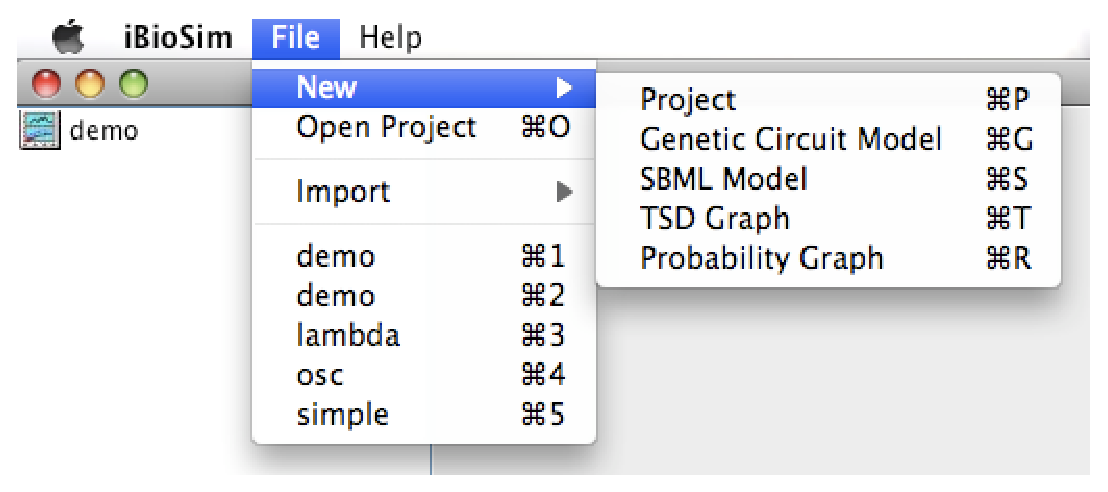
\includegraphics[height=80mm]{screenshots/newModel}
\end{center}

\begin{center}
\includegraphics[height=25mm]{screenshots/ModelId}
\end{center}

\begin{center}
\includegraphics[height=80mm]{screenshots/ModelEditor}
\end{center}

To add a chemical species, select the Add Species icon \includegraphics{../gui/icons/modelview/add_species_selected} and click on the schematic canvas.  This will drop a new species with default ID and other values.  You may change these defaults by double-clicking on the species to open the Species Editor.  In this case, let us change the ID to CI and units to mole.  We will leave all other values at their default values.  One thing that is important to note is that when this model is analyzed a default degradation reaction will be created which has a rate of 0.0075.  If you do not want a degradation reaction, you must change ``default'' to ``custom'' and change the degradation rate to 0.

%% TODO: remove mole setting
\begin{center}
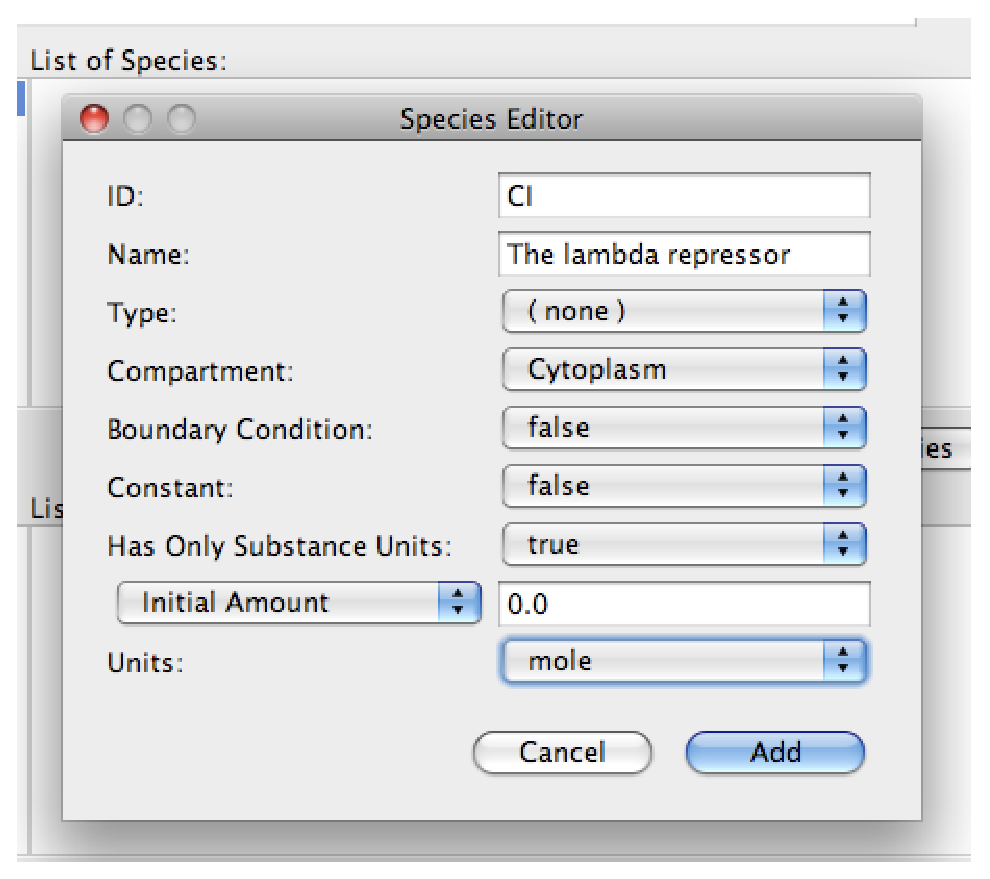
\includegraphics[height=80mm]{screenshots/species}
\end{center}

Add another species for the CI dimer molecule.  Edit this species to set its ID to CI2 and change its units to mole.  This species is created using a complex formation reaction with an equilibrium constant of 0.1 M$^{-1}$.  Change default to custom for the complex formation rate and set it to this rate as shown below.

%% TODO: remove mole setting
\begin{center}
\includegraphics[height=80mm]{screenshots/species2} 
\end{center}

The next step is to add a complex formation reaction to convert CI monomers into CI dimers.  Select the complex formation icon \includegraphics{../gui/icons/modelview/bio_activation_selected}, highlight the CI species, and while holding the mouse button stretch the complex formation arc to the CI2 species.   If you double click on the complex formation arc, an influence editor will open which indicates that this is a complex formation arc and the stoichiometry of binding (i.e., the number of molecules of the source species used to construct the sink species) is 2.  The default in this case is correct as it does take two molecules of CI to make CI2.

\begin{center}
\includegraphics[height=60mm]{screenshots/complex} 
\end{center}

Next, let's add the PR promoter which initiates transcription of the gene that produces the protein CII.  To do this, select the promoter icon \includegraphics{../gui/icons/modelview/promoter_mode_selected}, and click on the schematic canvas to drop the promoter with a default ID and parameter values.  Double click on the promoter to bring up the promoter editor.  Change the ID to PR and customize the RNAP binding equilibrium to be 0.69422, as well as, the open complex production rate to be 0.014. 

\begin{center}
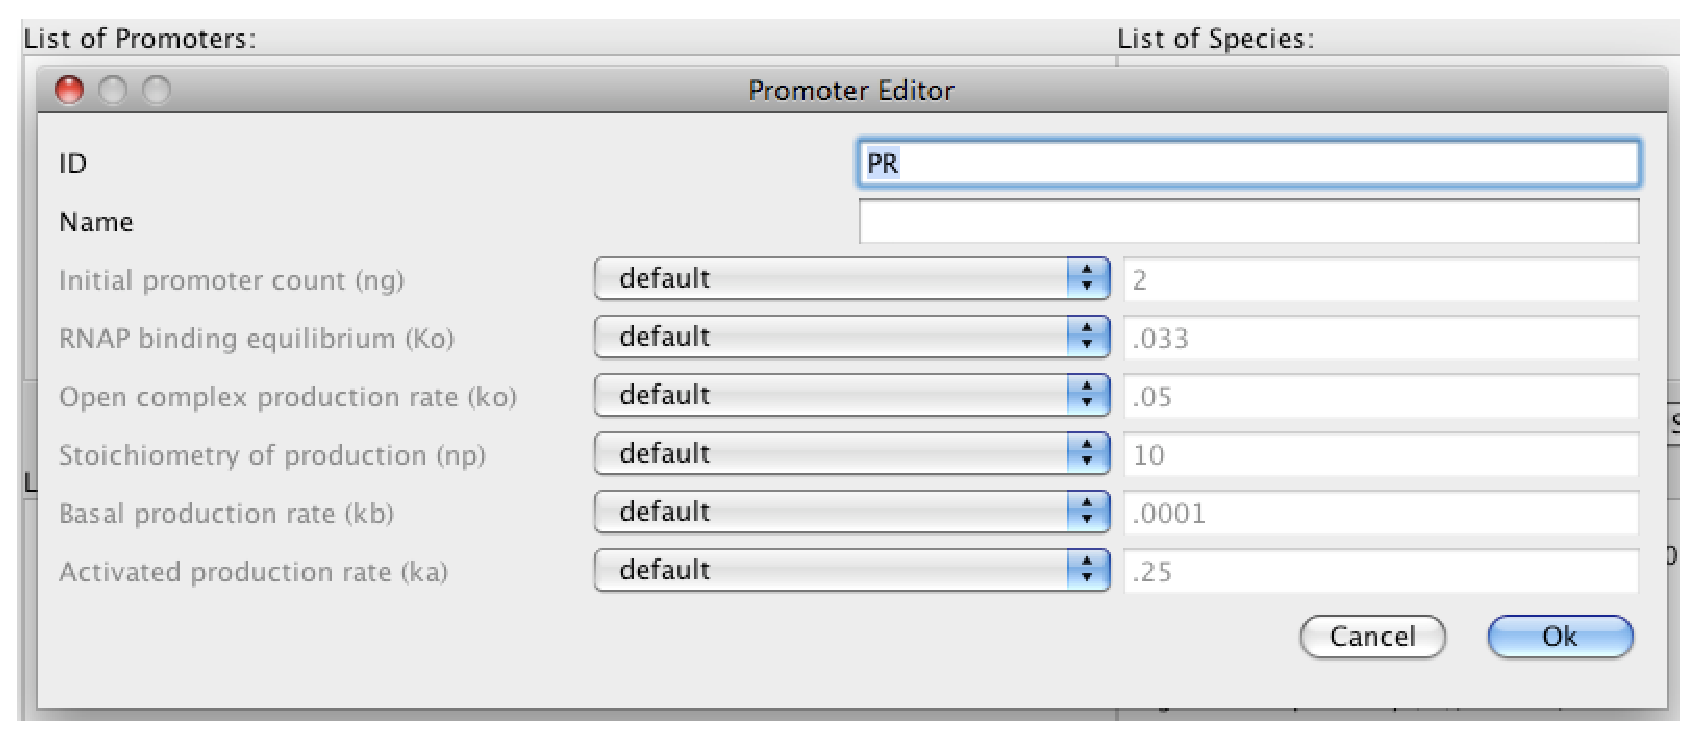
\includegraphics[height=80mm]{screenshots/promoter} 
\end{center}

The PR promoter is repressed by the CI2 species.  To create this relationship, select the repression arc icon 
\includegraphics{../gui/icons/modelview/inhibition_selected}, highlight the CI2 species, and while holding the mouse button stretch the repression arc to the PR promoter.  Next, double click on the repression arc to bring up the influence editor.  In this editor, customize the stoichiometry of binding to 1 indicating that just one CI dimer is necessary to repress this promoter and change the repression binding equilibrium to 0.2165.

\begin{center}
\includegraphics[height=60mm]{screenshots/repression} 
\end{center}

As mentioned earlier, the PR promoter initiations the production of the CII species.  Add the CII species following the steps given earlier for adding a species.  Then, highlight the PR promoter and while holding the mouse button stretch the production arc to the CII species.  Note that the icons selected for this are not important because all arcs from promoters to species are always production arcs.

\begin{center}
\includegraphics[height=80mm]{screenshots/production}
\end{center}

Finally, CII species activates the production of the CI species from the PRE promoter.  Promoters do not need to always be drawn.  They can also be implicit on an influence.  To add an activation arc with an implicit promoter, select the activation arc icon \includegraphics{../gui/icons/modelview/activation_selected}, highlight the CII species, and while holding the mouse button stretch the activation arc to the CI species.  This creates not only the influence but also a default promoter.   Double click on the activation arc to bring up the influence editor.  In this editor, customize the stoichiometry of binding to 1 indicating that just one CII molecule is necessary to activate this promoter and change the activation binding equilibrium to 0.00161.  Finally, click on the edit promoter button and change the ID of this promoter to PRE.  Also, customize the RNAP binding equilibrium to be 0.01, the basal production rate to be 0.00004, and the activated production rate to be 0.015.

\begin{center}
\includegraphics[height=80mm]{screenshots/activation}
\end{center}

\begin{center}
\includegraphics[height=80mm]{screenshots/activated_promoter}
\end{center}

%% TODO: ADD COMPARTMENT
% Highlight the {\tt default} compartment, select {\tt Edit Compartment}, and change its ID to {\tt Cytoplasm}.  Also, change the units to {\tt volume}.

%% TODO: ADD DEFINITIONS
% Select {\tt Definitions/Types} tab, and select {\tt Add Unit} and enter {\tt per\_second} as the ID.  Select {\tt Add to List},  select {\tt second} as the kind, change the exponent to $-1$,  and click {\tt Add}.  Click {\tt Add} in the {\tt Unit Definition Editor}.   Repeat these steps to create a {\tt per\_second\_mole} unit  (i.e., (second)$^{-1}$(mole)$^{-1}$).

\begin{center}
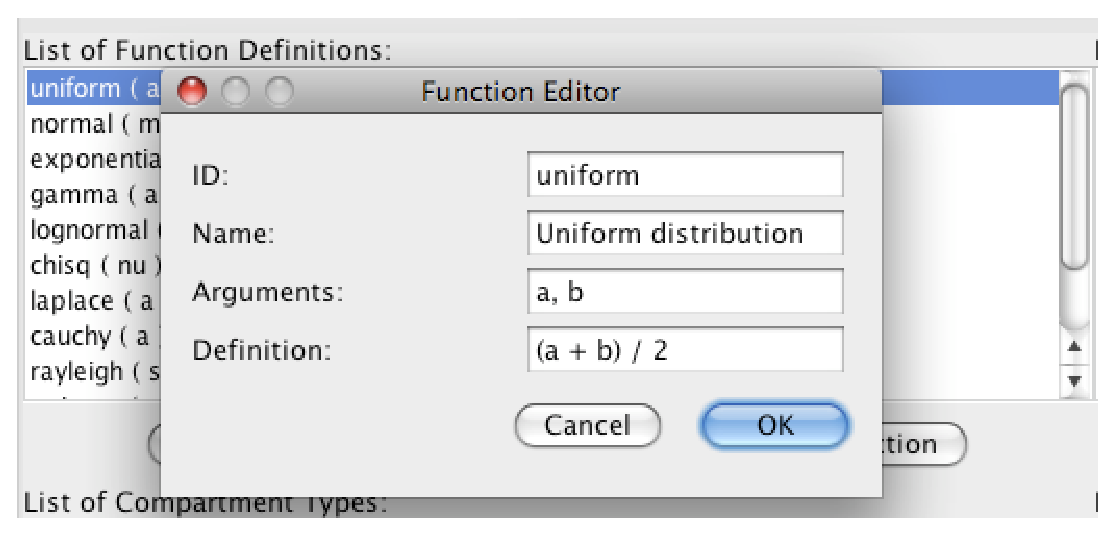
\includegraphics[height=70mm]{screenshots/function}
\end{center}

%% TODO: define nanomoles and microliters and set to model units
\begin{center}
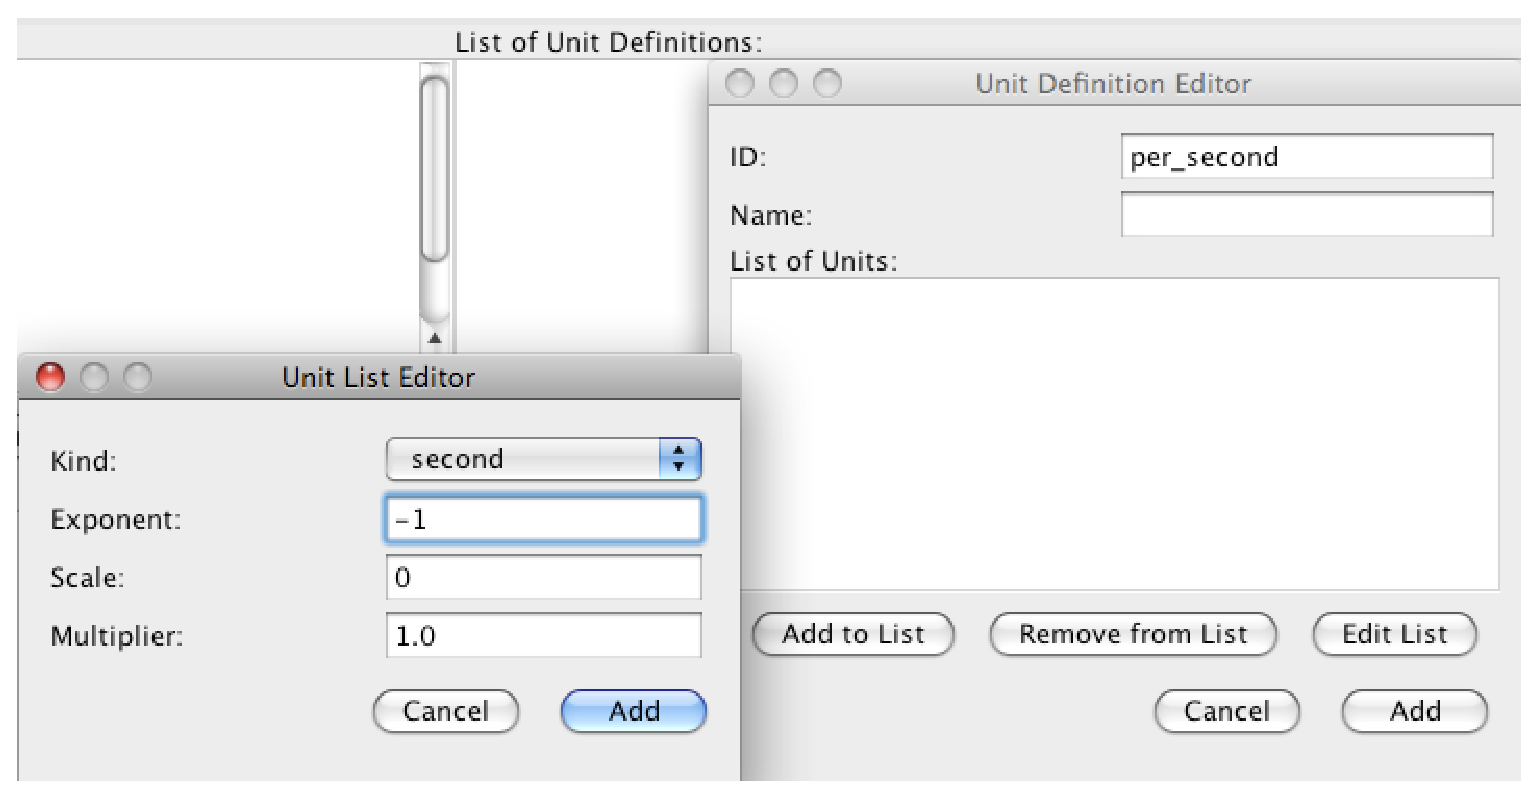
\includegraphics[height=70mm]{screenshots/units}
\end{center}

\begin{center}
\includegraphics[height=70mm]{screenshots/ModelUnits}
\end{center}

%% TODO: remove liter units
\begin{center}
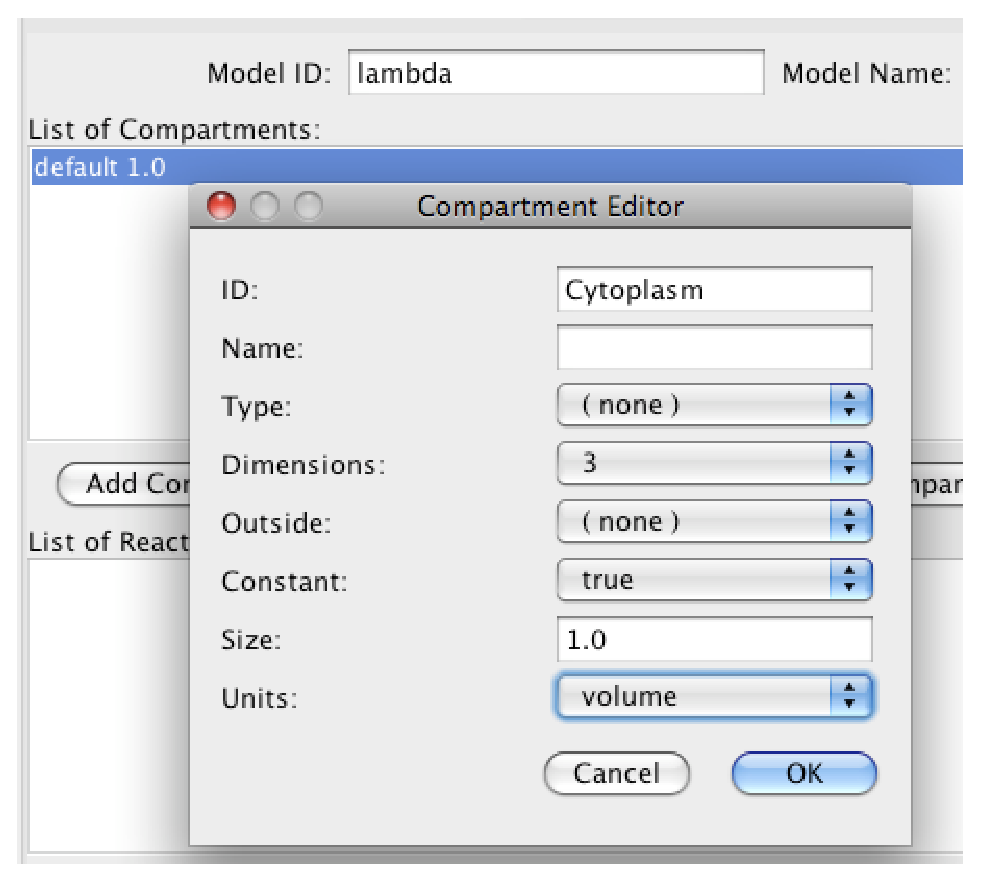
\includegraphics[height=65mm]{screenshots/compartment}
\end{center}

% The next item on the toolbar is a checkbox used to indicate if the model is to be considered enclosed within a \emph{compartment}.  The combo box is used to select the enclosing compartment for the model.  

%% TODO: ADD PARAMETER
% Select {\tt Add Parameter} and enter {\tt nd} as the ID, {\tt Number of molecules in dimer} as the name, the value to be 2, and change the units to {\tt dimensionless}.

\begin{center}
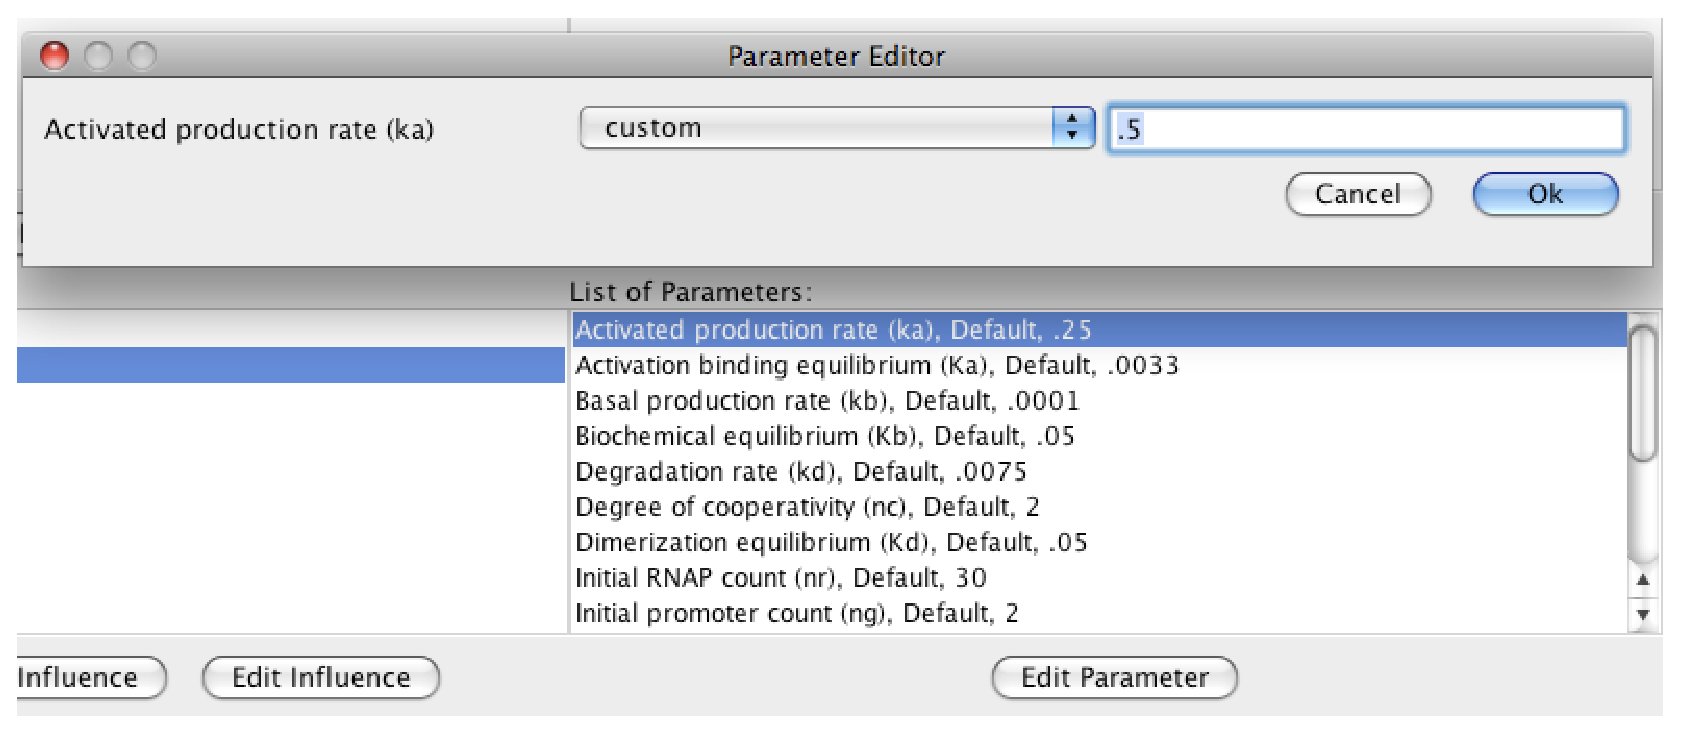
\includegraphics[height=65mm]{screenshots/GCMparam}
\end{center}

\begin{center}
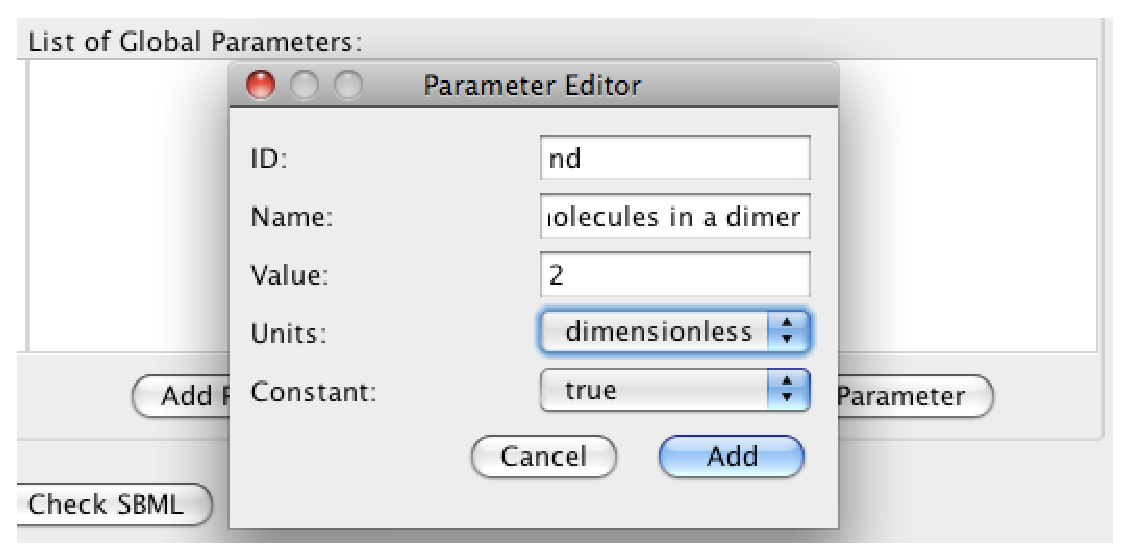
\includegraphics[height=65mm]{screenshots/parameter}
\end{center}

\begin{center}
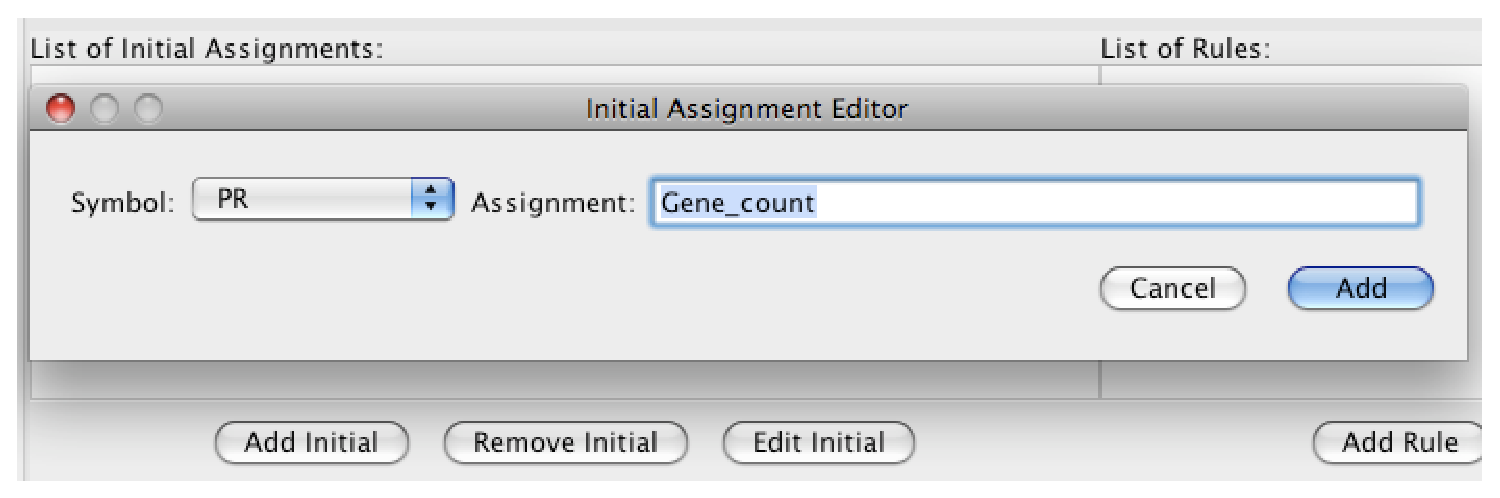
\includegraphics[height=80mm]{screenshots/initial}
\end{center}

\begin{center}
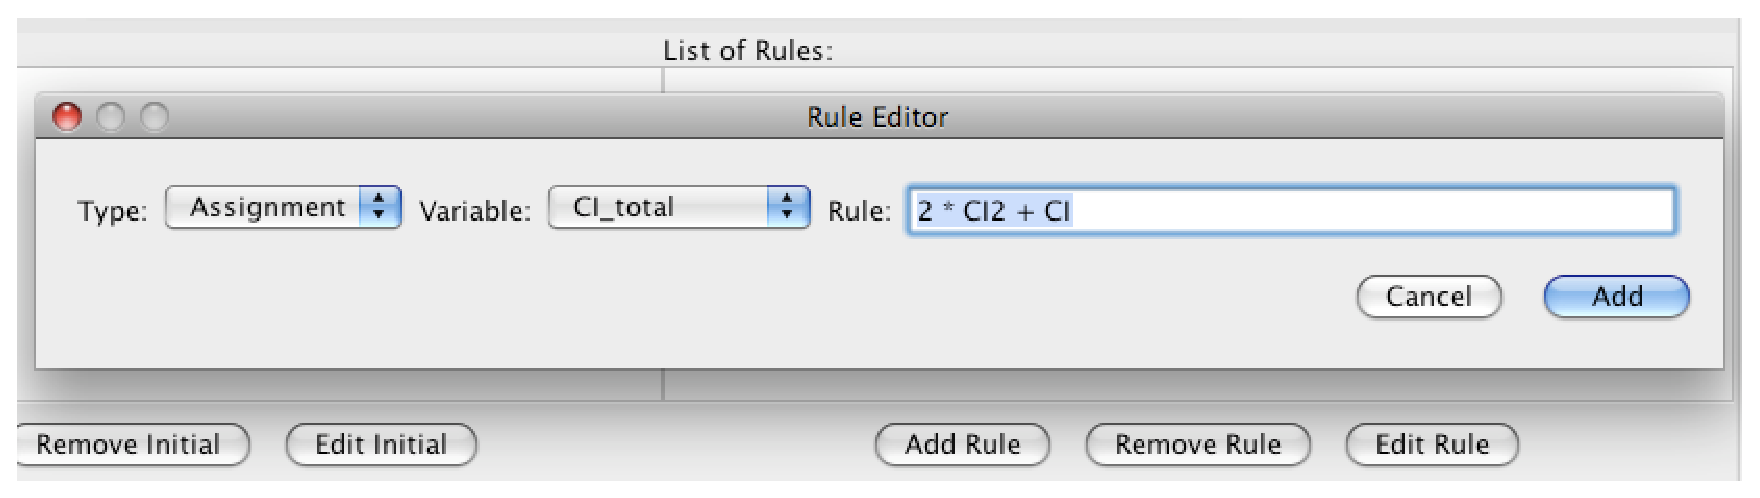
\includegraphics[height=80mm]{screenshots/rule}
\end{center}

%% TODO: add properties/constraints
%% TODO: add events

At this point, make sure your model has been saved by either clicking on the Save icon \includegraphics{../gui/icons/save} or selecting the Save option from the File menu.

\section{Analysis Tool}

This section describes how to analyze the model just created.  The first step is to create an analysis view.  To do this, right click on the model file and select Create Analysis View.  Enter the analysis ID {\tt simLambda}.  At this point, a new analysis view should open.  You should also notice that an icon appears next to your model file.  When you click on this, it will show you all of the analysis and learn views associated with this model.

\begin{center}
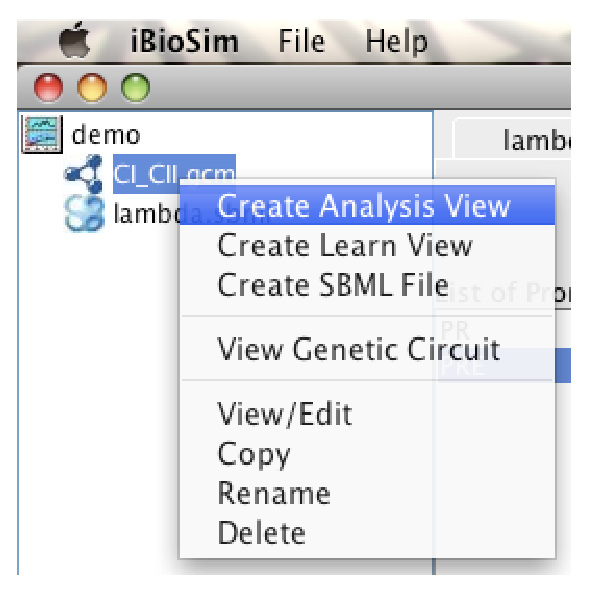
\includegraphics[height=60mm]{screenshots/GCMAnalysis}\\
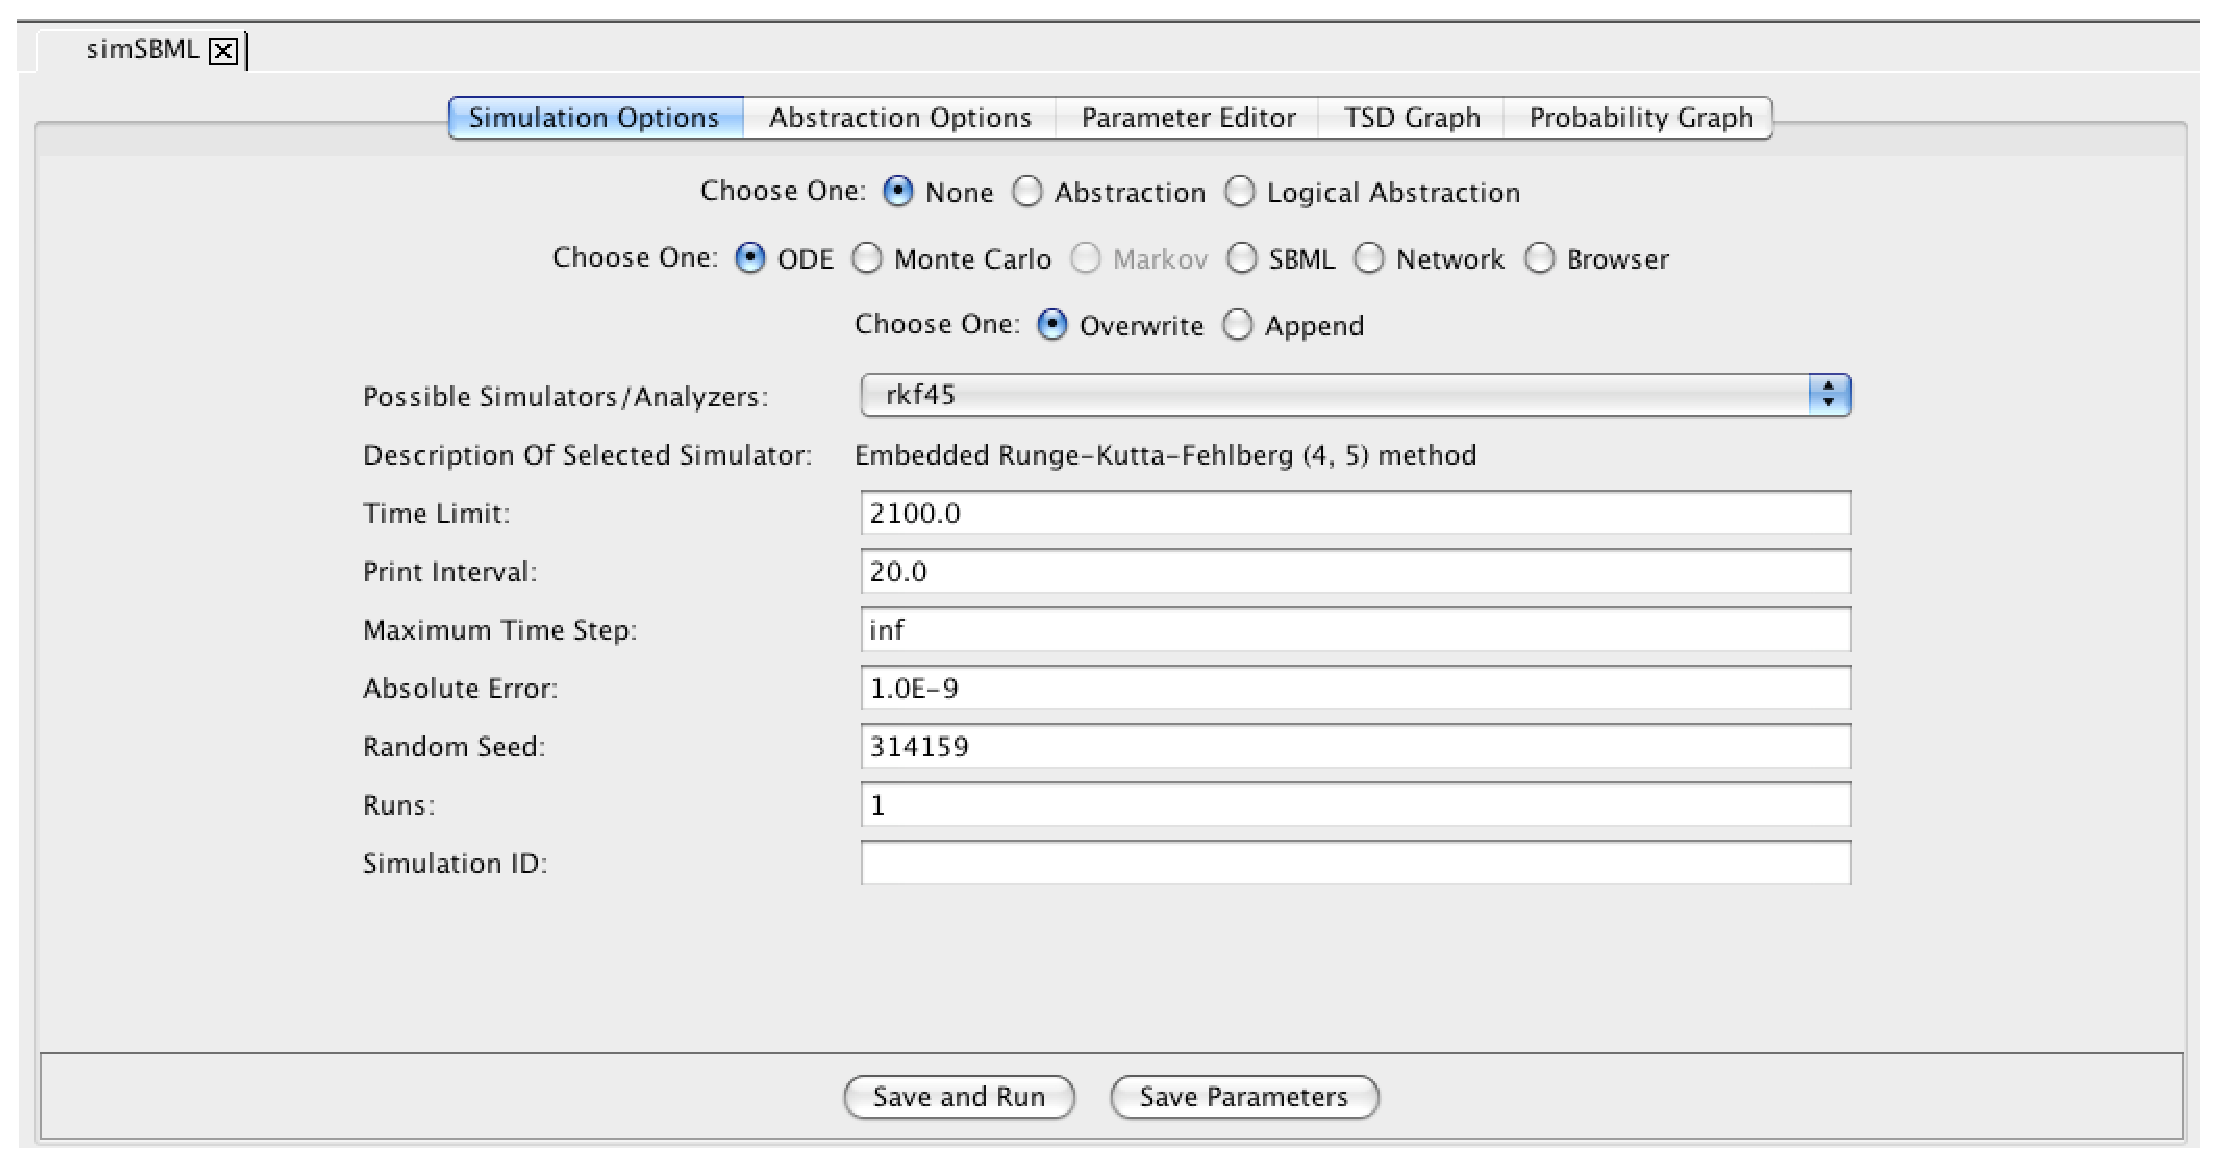
\includegraphics[height=90mm]{screenshots/analysisView}
\end{center}

In order to perform analysis, the analysis tool first converts the model into a reaction-based model in the \emph{Systems Biology Markup Language} (SBML).  There are three different ways to see the reaction-based model that is produced.  If GraphViz is installed on your computer, you can select Network for your Simulation Type.  Then, either press the Save and Run icon \includegraphics{../gui/icons/run-icon} or select the Save and Run option from the File menu.  The result will be a GraphViz window will open showing the reaction-based model such as the one shown below for our example.  If it does not open in GraphViz, make sure that you have files with the {\tt .dot} file extension associated with GraphViz on your computer.  You can also view the model in a web browser by selecting Browser for your simulation type.  In this case, you should ensure that you have files with the {\tt .xhtml} extension associated with your favorite browser.  Finally, you can save the reaction-based model by selecting Model as your simulation type.  In this case, you must provide a new model ID.  This new model will appear in your project, and it can be opened in the Model Editor.  Since this model does not include any layout information, you will need to either lay it out by hand or using one of the default layout routines selectable using the Apply Layout icon \includegraphics{../gui/icons/modelview/choose_layout_selected},

\begin{center}
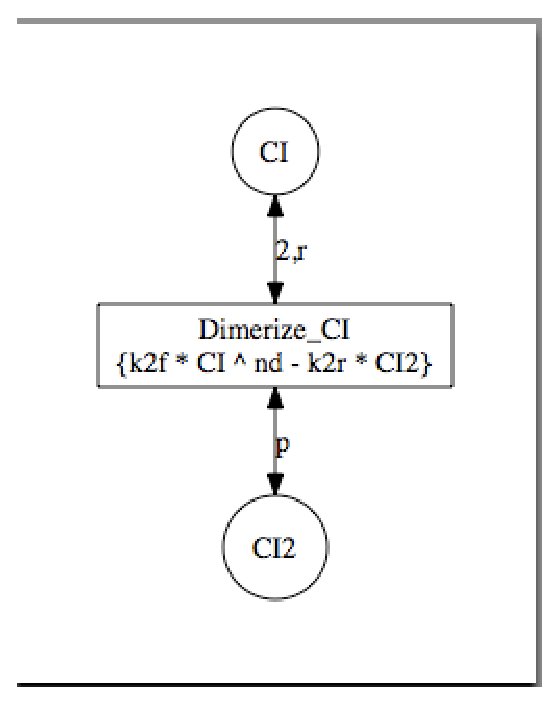
\includegraphics[height=80mm]{screenshots/viewNetwork}
\end{center}

\begin{center}
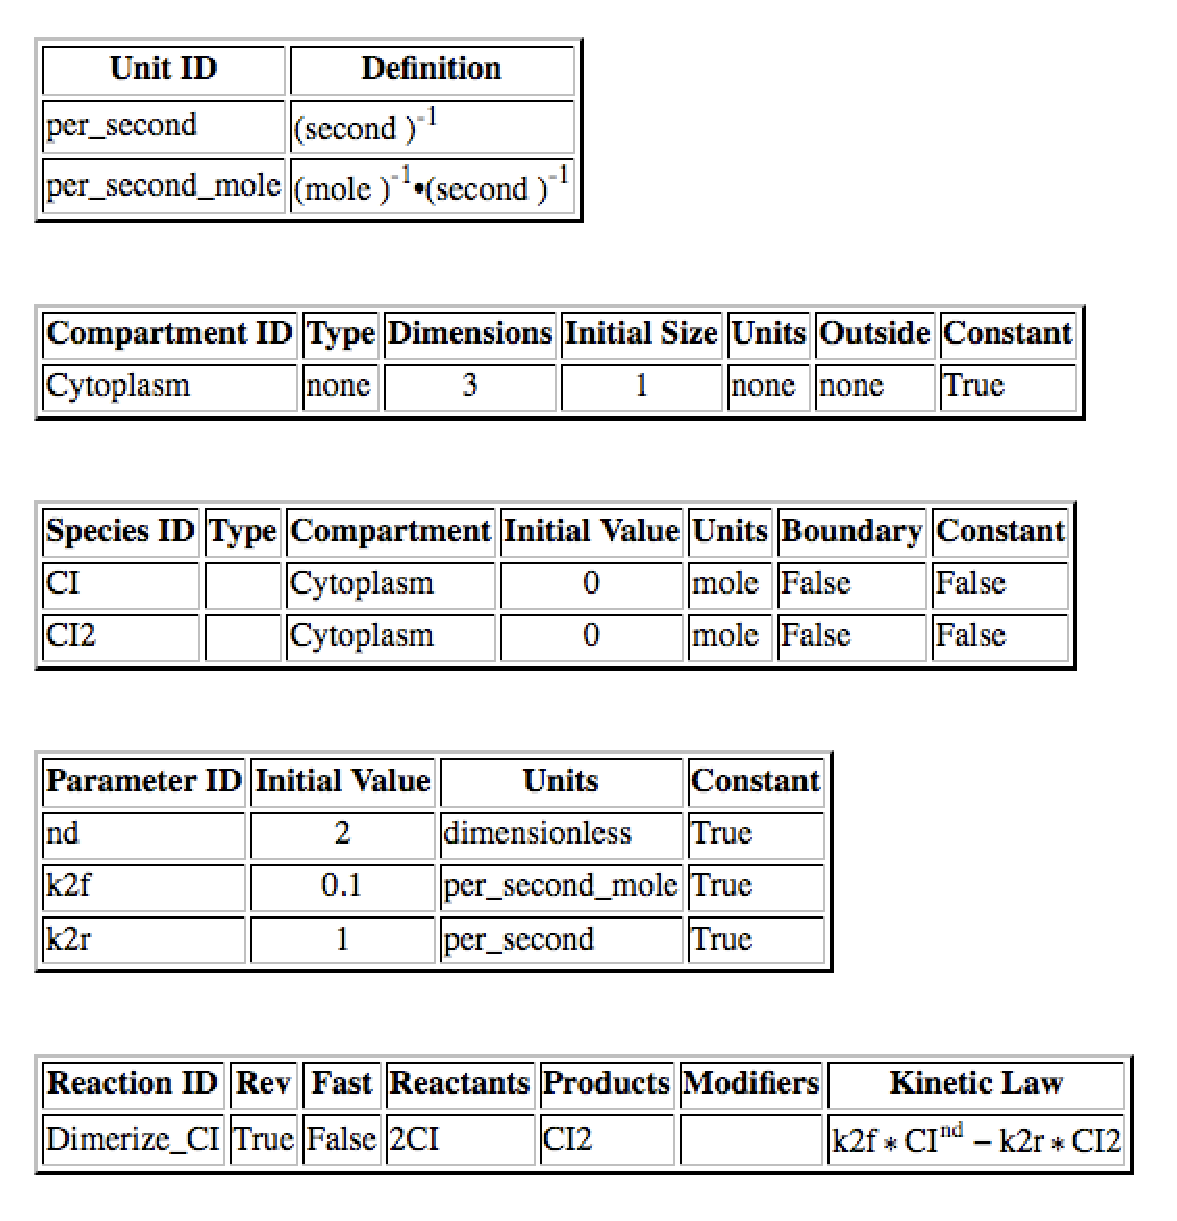
\includegraphics[height=110mm]{screenshots/viewBrowser}
\end{center}

\begin{center}
\includegraphics[height=80mm]{screenshots/reactionModel}
\end{center}

Next, click on the SBML elements tab.  This tab allows you to select which SBML model elements to include in your analysis.  This includes initial assignments, rules, constraints, and events.  Initially, let's only include the rule to compute CI\_total.  Uncheck all the elements.

\begin{center}
\includegraphics[height=80mm]{screenshots/SBMLElements}
\end{center}

Now, go back to the simulation options tab.  Here, change the simulation type back to ODE, change the time limit to 2100.0, change the print interval to 10.0, and enter a Simulation ID of {\tt ode}.  Then, either press the Save and Run icon \includegraphics{../gui/icons/run-icon} or select Save and Run option from the File menu.
After the simulation completes, click on the TSD Graph tab.  Double click on the graph to bring up the graph editor.
Open the {\tt ode} simulation, highlight Average, select CI\_total and CII, change the Title to ``ODE Simulation Results'', change the X-Axis Label to ``Time (seconds)'', and change the Y-Axis Label to ``Number of Molecules''.  
Press the OK button.  
 
\begin{center}
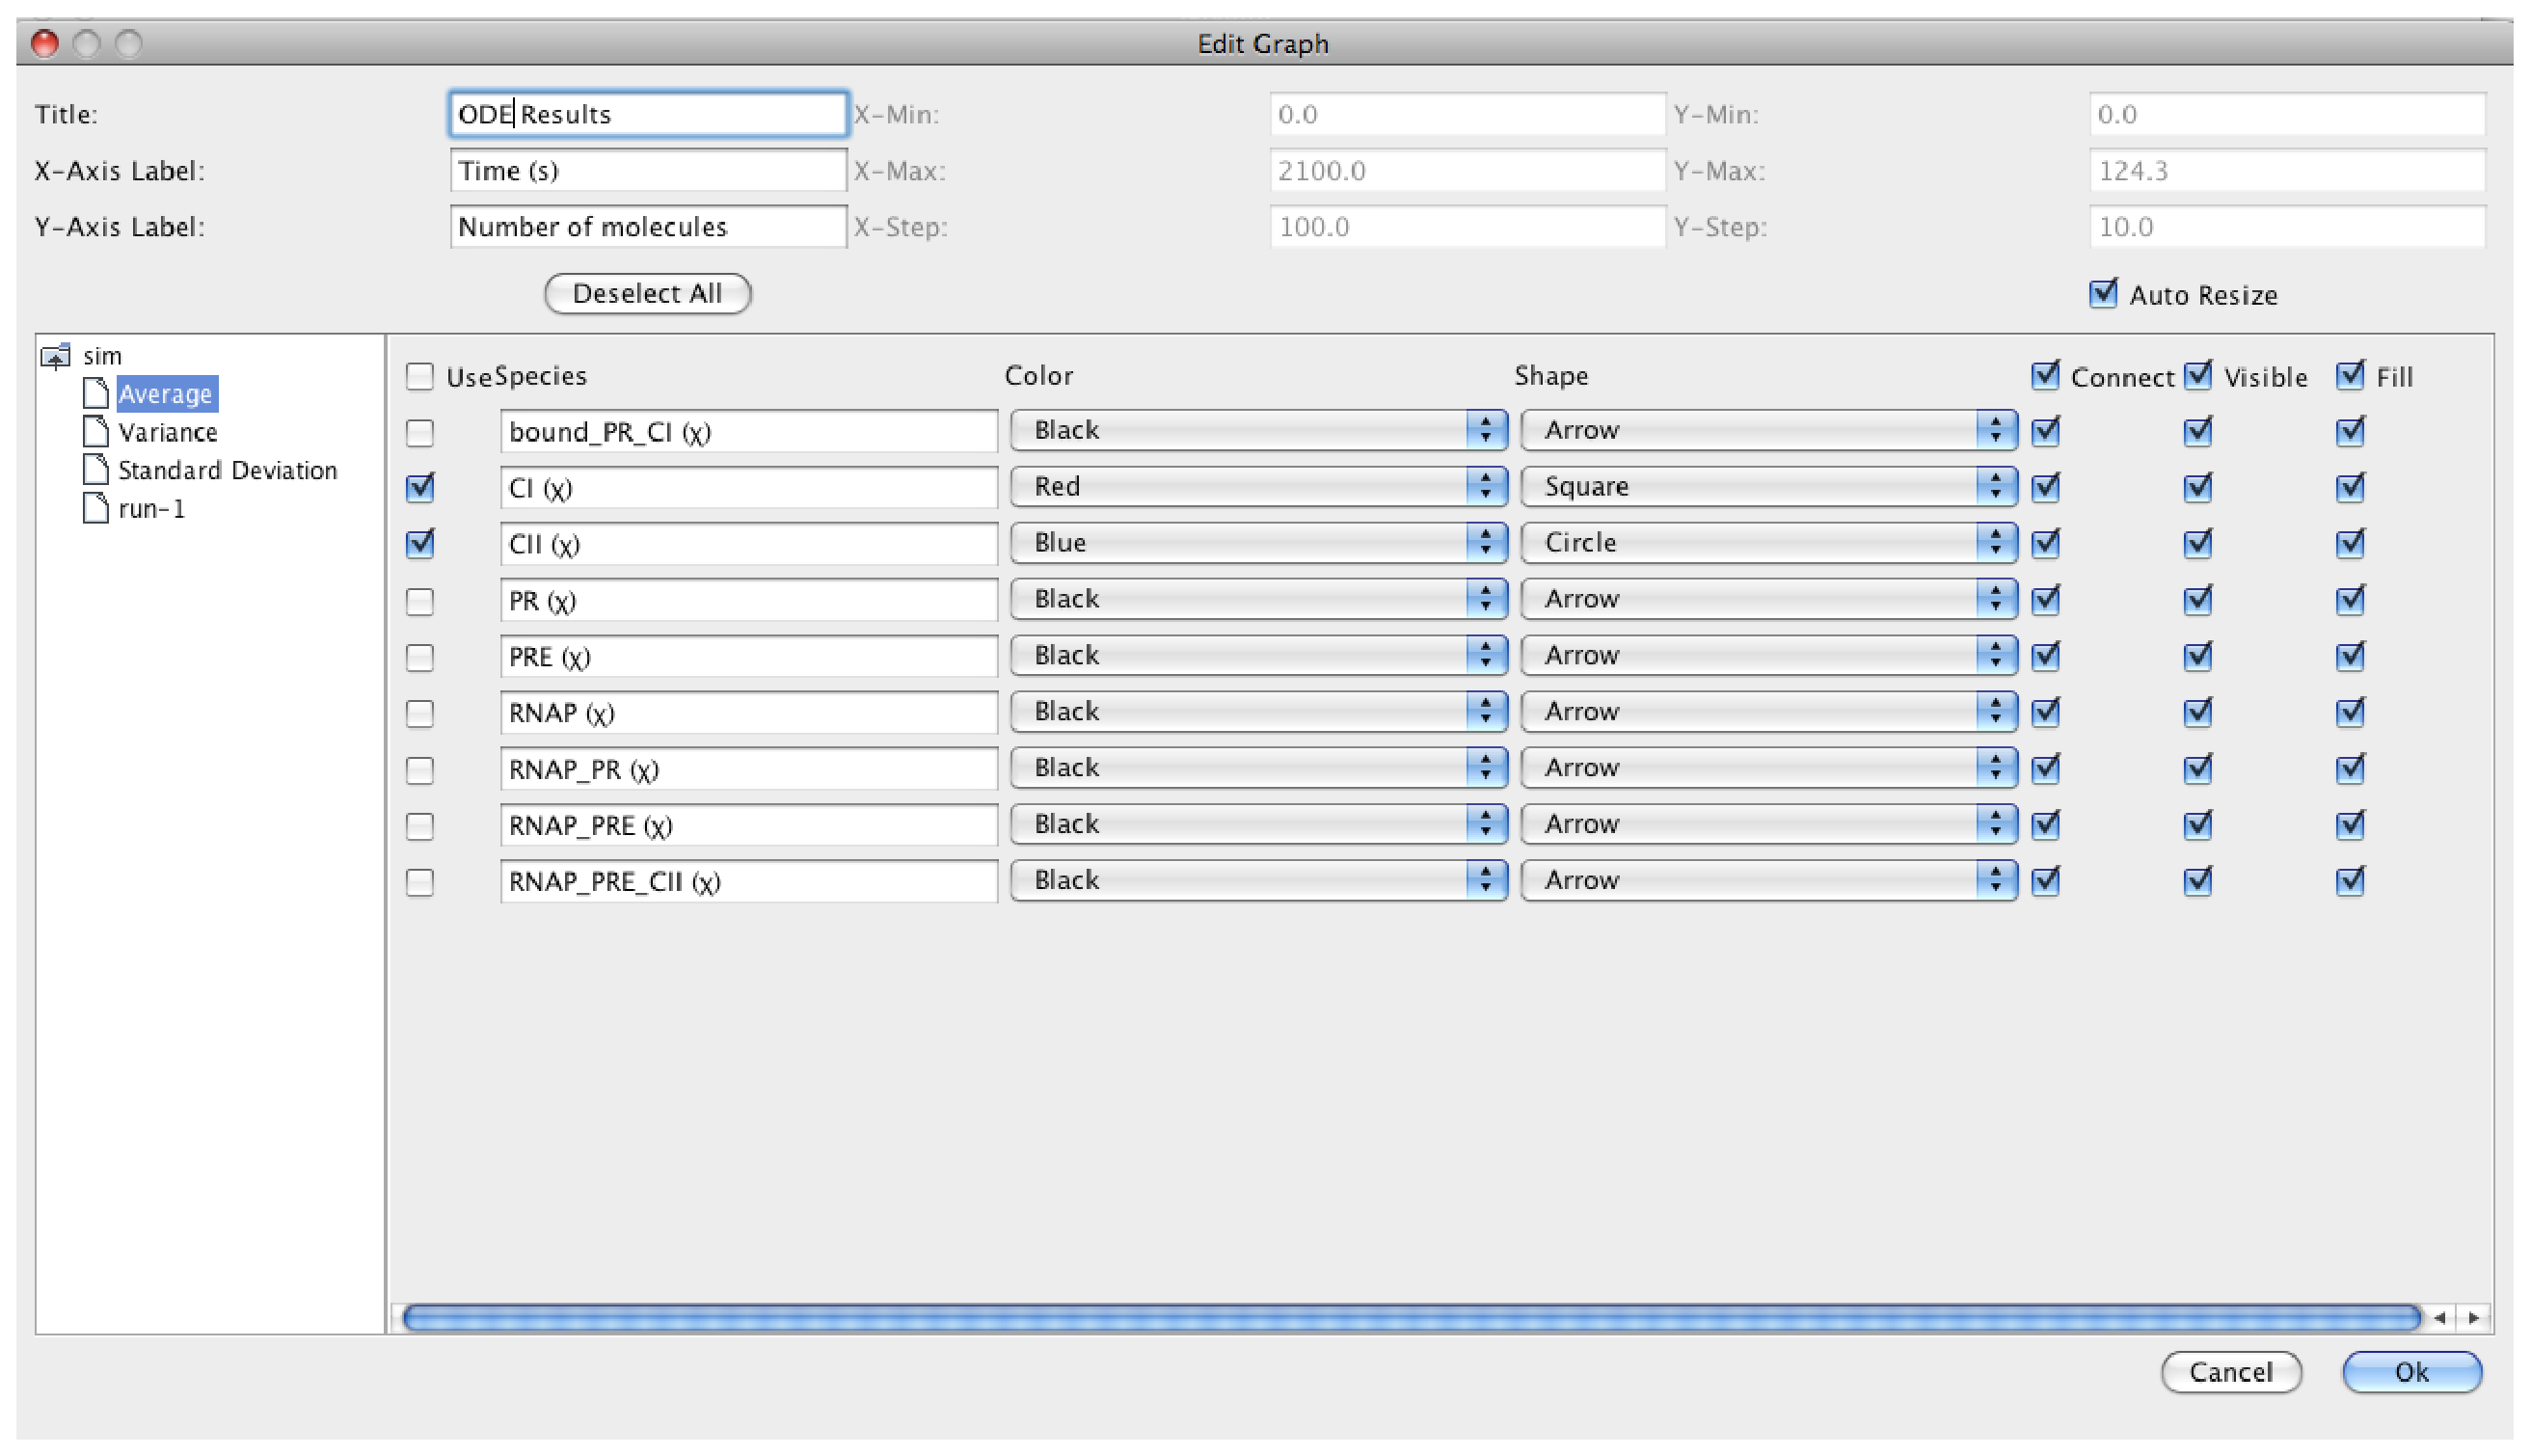
\includegraphics[height=90mm]{screenshots/odeResults}\\
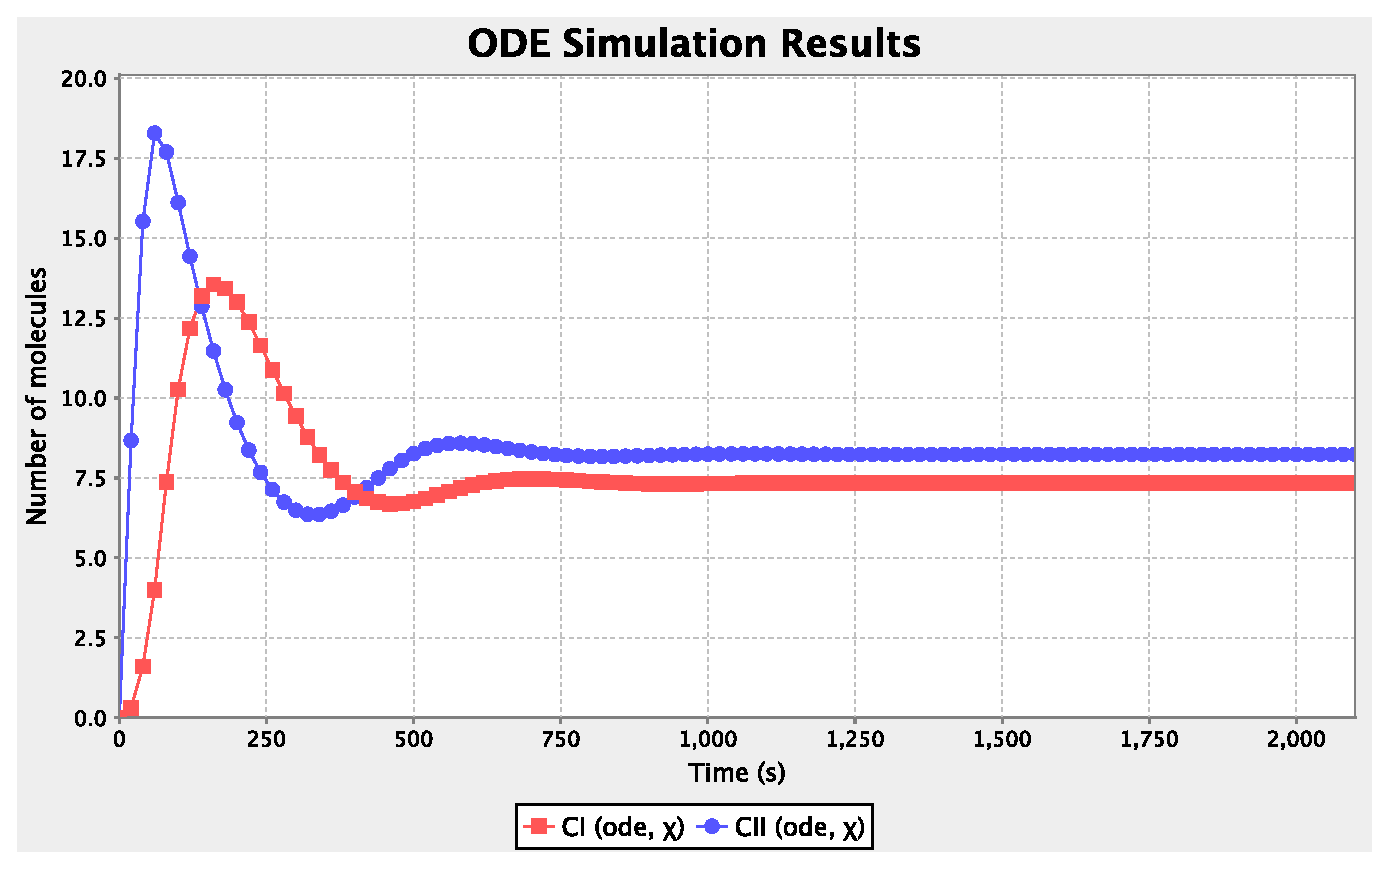
\includegraphics[height=80mm]{screenshots/odeSimResults}
\end{center}

Graphs can be exported in a variety of formats including:
\begin{itemize}
\item Time series data format (TSD).
\item Comma separated value (CSV).
\item Column separated data (DAT).
\item Encapsulated postscript (EPS). 
\item Joint Photographic Experts Group (JPG). 
\item Portable document format (PDF).
\item Portable network graphics (PNG). 
\item Scalable vector graphics (SVG).
\end{itemize}
In order to export a graph, you can either click on the Export icon \includegraphics{../gui/icons/export} or select one of the graph export options from the File menu.  When using the Export icon, the type of file exported will depend on the extension provided to the file name.  Click on the Export icon, browse to a location on your file system and enter the file name of {\tt ode.pdf} to create a PDF file for your graph.

\begin{center}
\includegraphics[height=60mm]{screenshots/exportTSD}
\end{center}

Now, select the Simulation Options tab again, select {\tt Monte Carlo}, change the number of runs to 100, set the simulation ID to {\tt ssa}, and click on the Save and Run icon.  Click on the TSD Graph tab.  Double click on the graph to bring up the graph editor.  Open the {\tt ssa} simulation directory, and highlight {\tt run-1}.
Select CI\_Total and CII, change the title to ``SSA Simulation Results'', change the X-Axis Label to ``Time (seconds)'', and change the Y-Axis Label to ``Number of Molecules''.  Press the OK button.  Click on the
Export icon and enter the file name {\tt ssa-1.pdf}.  Repeat these steps to generate graphs for the average ({\tt
  average.pdf}) and standard deviation ({\tt stddev.pdf}).  Note that you can use the ``Deselect All'' button to
remove all items from the graph.

\begin{center}
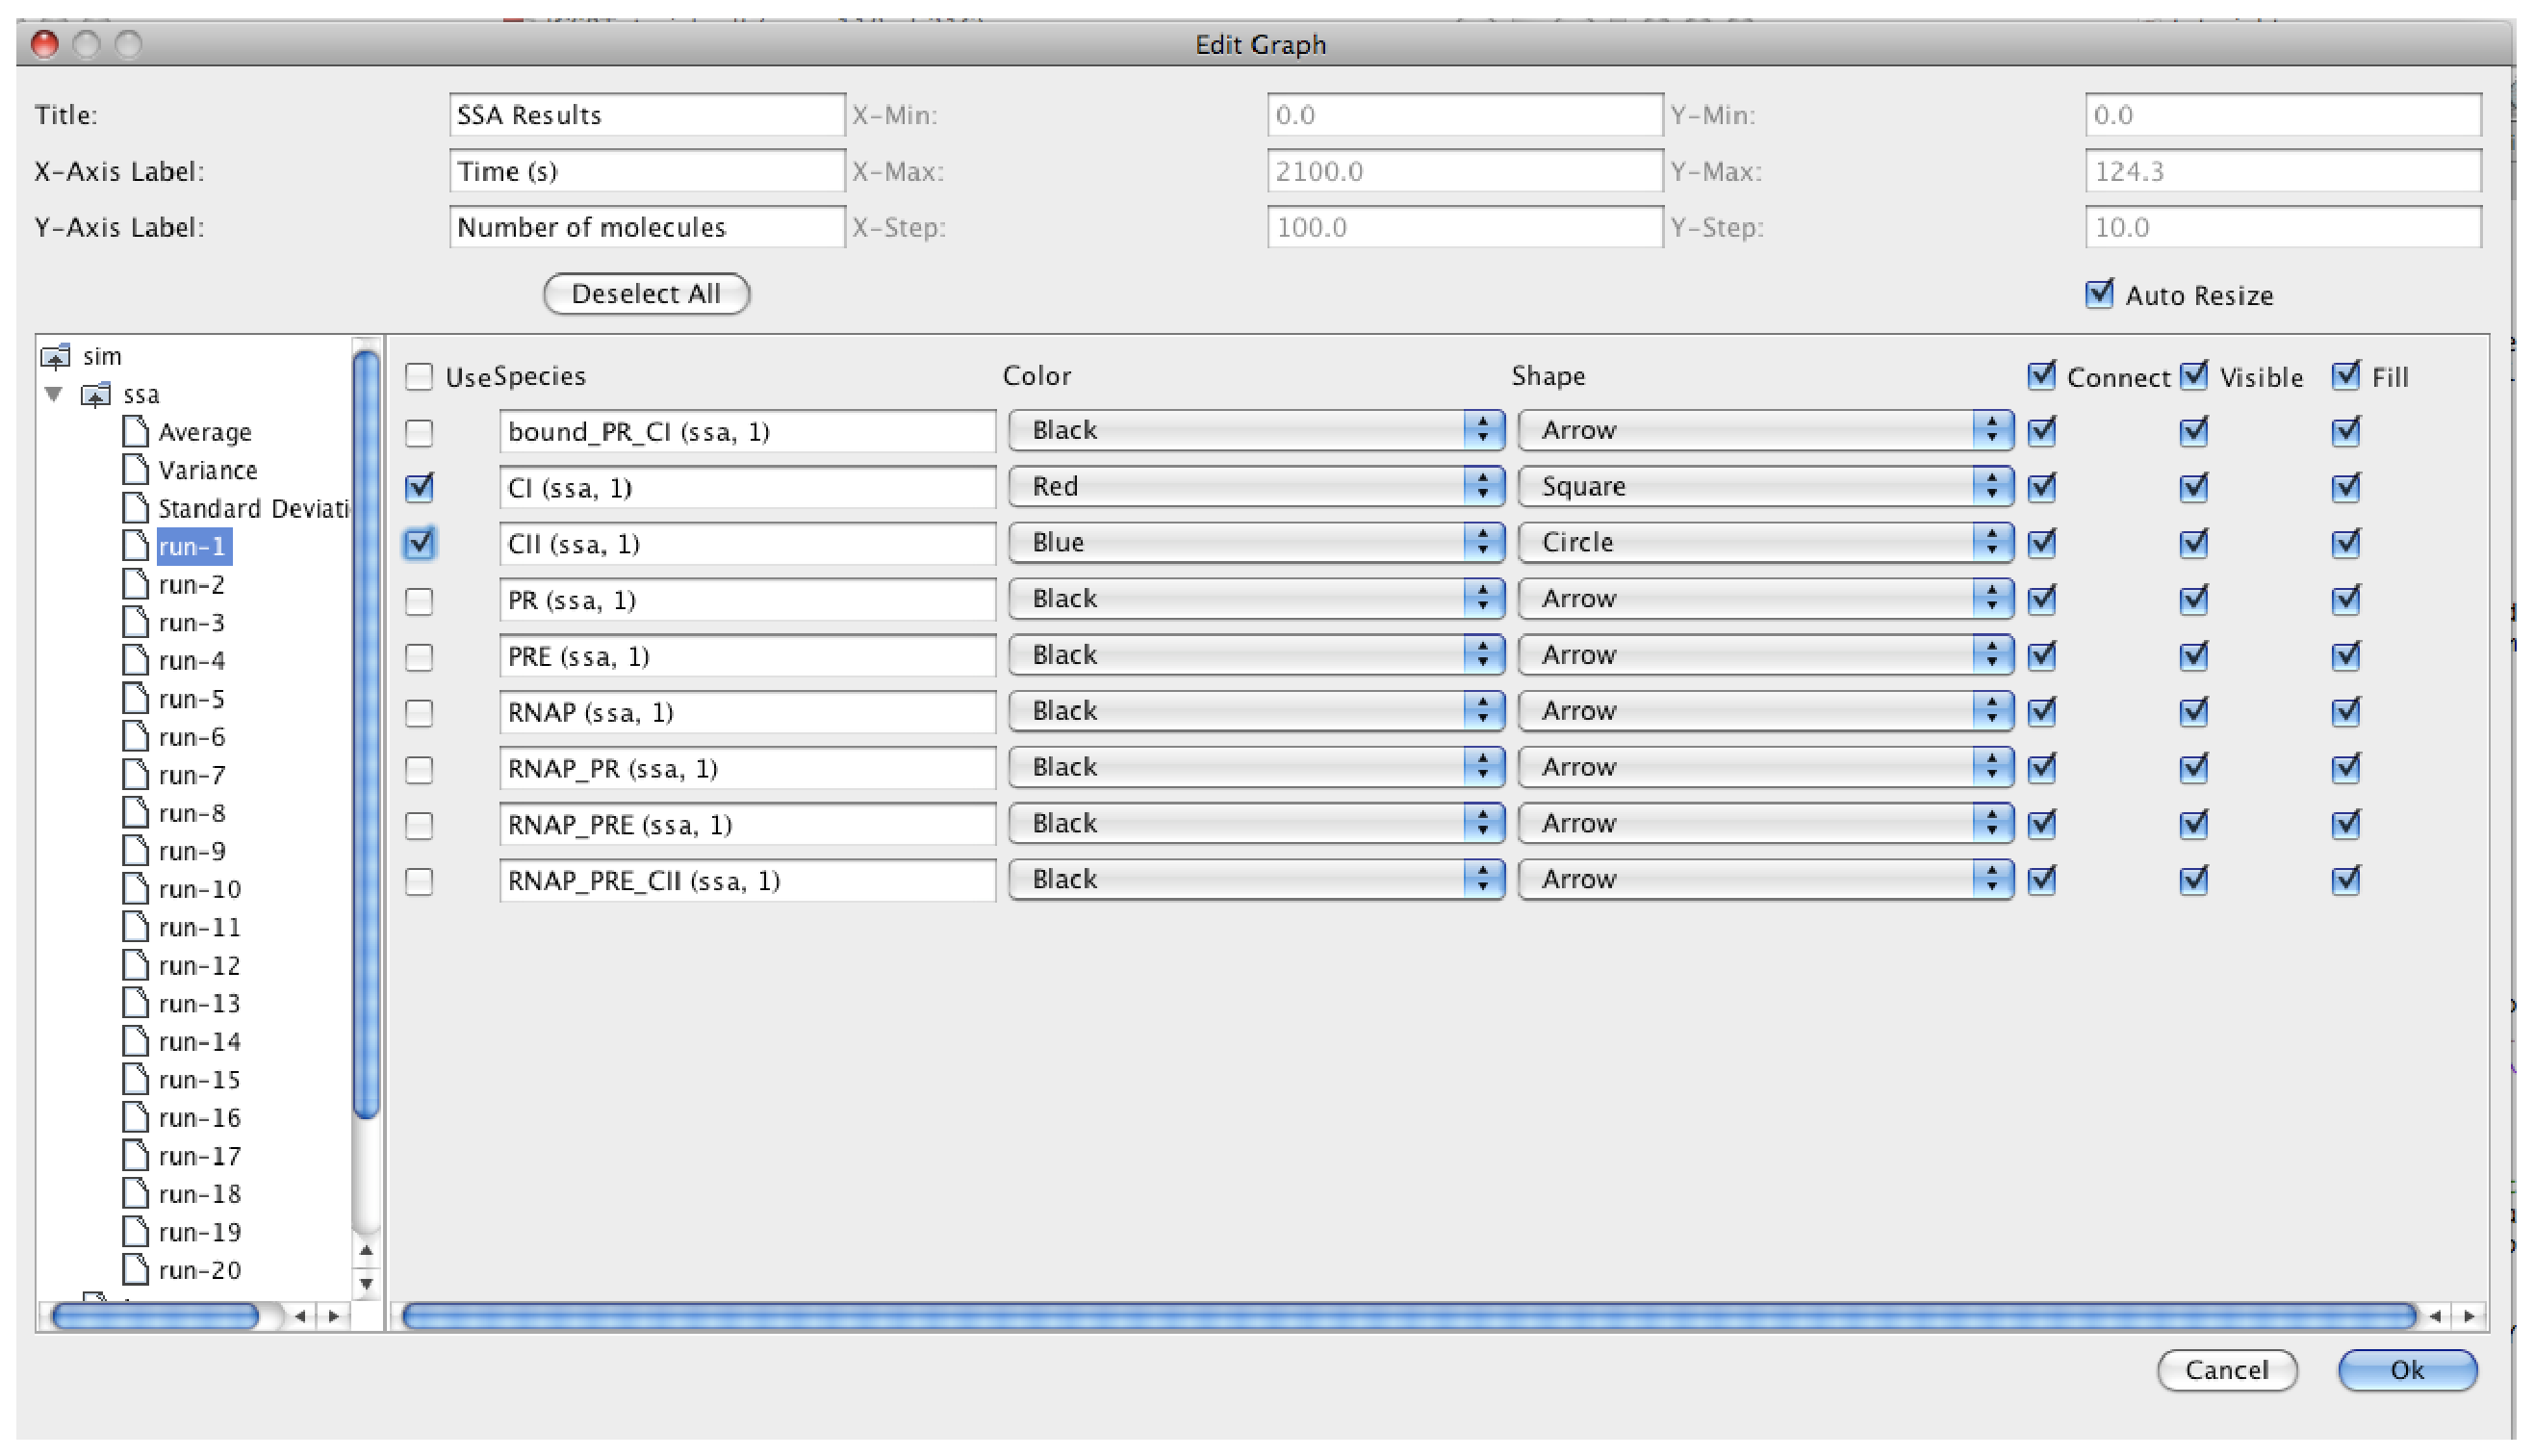
\includegraphics[height=90mm]{screenshots/ssaResults}\\
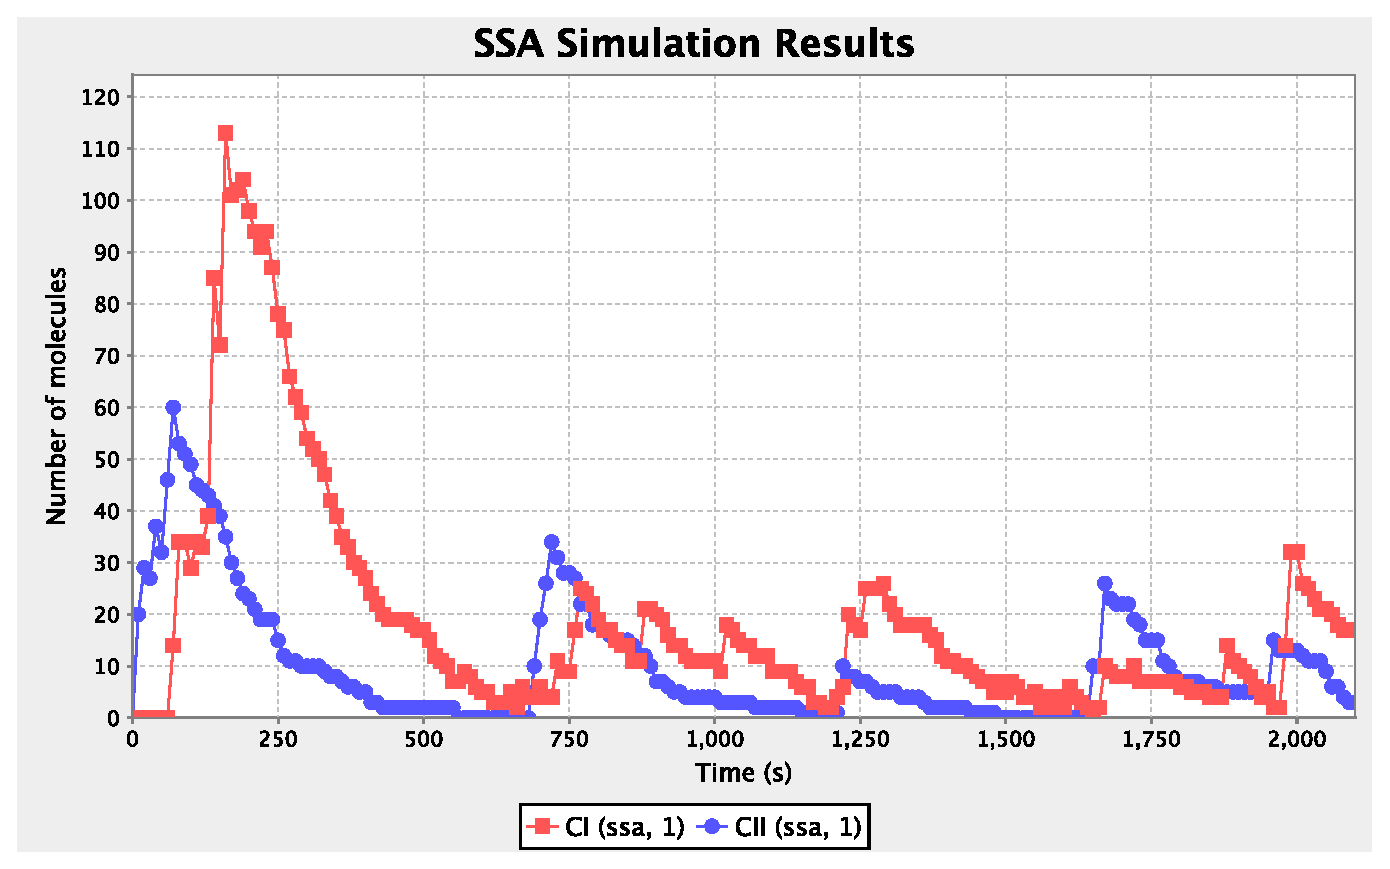
\includegraphics[height=80mm]{screenshots/ssaSimResults}
\end{center}

Another way to view simulation results is on the schematic.  To do this, click on the schematic tab.  At the bottom of the window, select the Choose Simulation button which brings up a window with all the simulations in this analysis view.  Open the {\tt ssa} directory, select {\tt run-1.tsd}, and press OK. 

\begin{center}
\includegraphics[height=80mm]{screenshots/chooseSim}
\end{center}

Now, click on the CI species which brings up the Edit Species window.  Select the Appearance tab.  Here you can select how you want the species to appear as you playback the simulation.  You can have it change color on a gradient, change size, or change opacity.  You can also select the range of molecule counts to use for the gradients.  Finally, you can indicate that these selections are either for this species or all species in the model.  For our example, let's make CI follow a green color gradient, CI2 follow a red color gradient, and CII follow a blue color gradient.
\begin{center}
\includegraphics[height=50mm]{screenshots/editSpeciesAppearance}
\end{center}

Once you have made your selections, you can now playback the simulation.  You can either single step the simulation by pressing the \includegraphics{../gui/icons/modelview/movie/single_step} icon or play continuously by pressing the \includegraphics{../gui/icons/modelview/movie/play} icon.  The playback can also be paused by pressing the \includegraphics{../gui/icons/modelview/movie/pause} icon and restarted by pressing the  \includegraphics{../gui/icons/modelview/movie/rewind} icon. 

\begin{center}
\includegraphics[height=80mm]{screenshots/movieView}
\end{center}

Using the schematic tab, you can also adjust initial values and parameters allowing one to perform simulations to determine the effect of these changes.  Clicking on any species, promoter, reaction, or influence brings up the corresponding editor.  To change a value, switch the corresponding combo box to modified which will then allow you to change the value.  For example, as shown below, we have reduced the degradation rate for CI to 0.00075.  Now, rerun the simulation and observe the change in the simulation data.

%% TODO: show results
\begin{center}
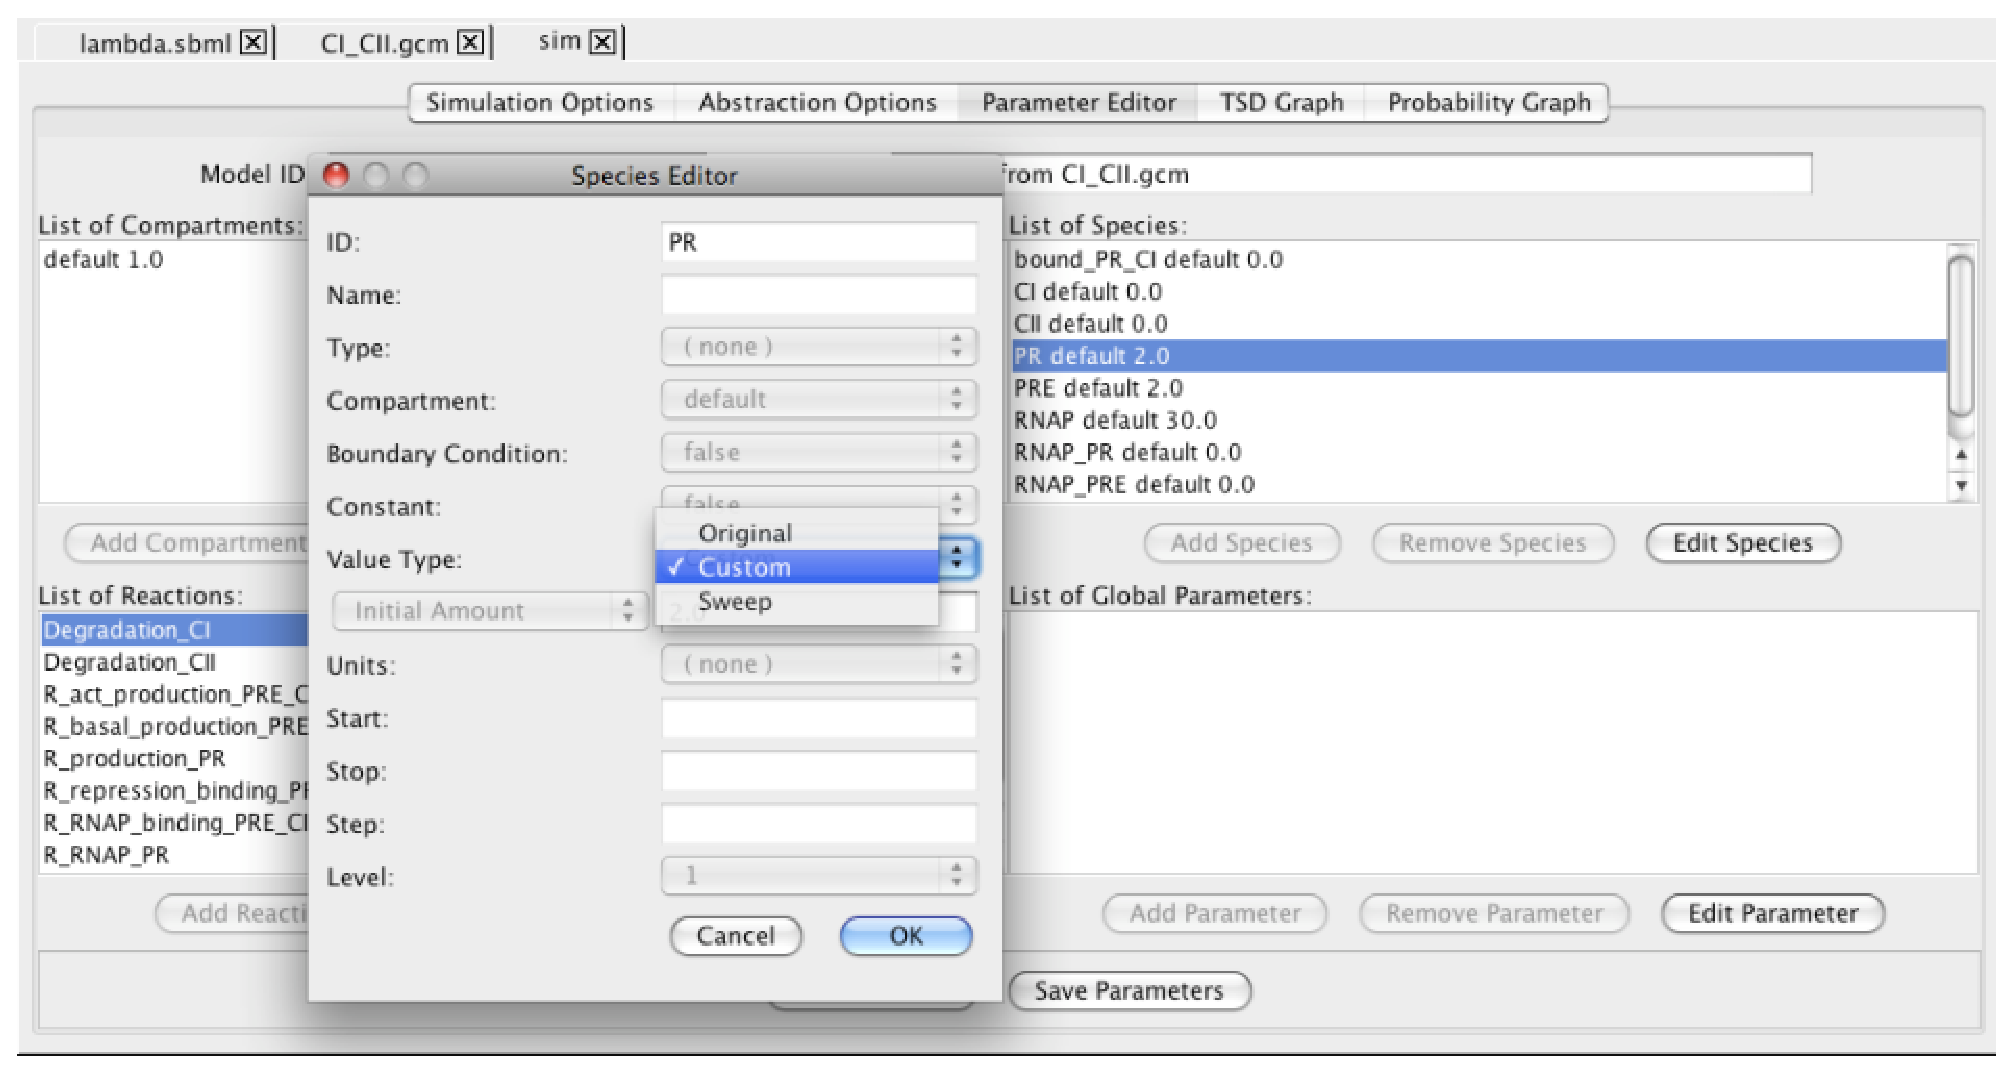
\includegraphics[height=50mm]{screenshots/paramEdit}
\end{center}

In addition to making single changes, you can also sweep a value as shown below.   When you click on the Sweep button, it brings up a window where you can select the start value, the stop value, and the step value.  In this example, simulations are generated using degradation rates of 0.001, 0.003, 0.005, and 0.007.  The level indicates how the sweep should perform when multiple variables are swept at the same time.  A variables at the same level are changed at the same time.  Furthermore, all variables on level 2 are stepped through all their values before changing the values of those variables on level 1.  After the values on level 1 are changed, the values on level 2 are stepped through all their values again.  Rerun the simulation and create a graph that shows the value of CI for each of the different degradation rates.

%% TODO: show results
\begin{center}
\includegraphics[height=50mm]{screenshots/sweep}
%\includegraphics[height=90mm]{screenshots/sweepPR}
\end{center}

The efficiency of simulation can be improved by employing various automatic abstraction techniques.  Go back to the Schematic tab and change the degradation rate of CI back to the default value.  Also, go to the SBML elements tab and uncheck the rule for CI\_total.  To activate abstraction, click on the Simulation Options tab, select Abstraction and change the simulation ID to {\tt abs}.  Press the Save and Run icon and note that the simulation time is substantially faster.  Plot both the SSA results for CI\_total and CII with the abstraction results for CI (note this is now equivalent to CI\_total after abstraction) and CII.

\begin{center}
\includegraphics[height=90mm]{screenshots/absResults}
\end{center}

One way to understand why abstraction is so much faster is by looking at the complexity of the reaction-based model before and after abstraction.  The reaction-based model after abstraction is shown below which is clearly much simpler than the full model shown earlier.

\begin{center}
\includegraphics[height=80mm]{screenshots/viewNetworkAbs}
\end{center}

\section{Learn Tool}

This section describes how a model can be learned from time series data using {\tt iBioSim}'s Learn Tool.  To demonstrate the Learn Tool, first create a simple model, {\tt lambdaLearn}, which just includes the two species CI and CII as shown below.  Next, create a learn view by right clicking on this model file and selecting Create Learn View.  Give this learn view the ID {\tt learnLambda}.  At this point, a new learn view should open.  You should also notice that an icon appears next to your model file.  When you click on this, it will show you all of the analysis and learn views associated with this model.

\begin{center}
\includegraphics[height=60mm]{screenshots/createLearn}
\end{center}

The next step is to add some experimental data from which you wish to learn a model.  In this demo, we will just utilize our simulation data as synthetic experimental data.  To do this, click Copy From View, and select {\tt simLambda/abs}.  Highlight {\tt simLambda/abs/run-1.tsd}, and you should see the simulation data for CI and CII appear on the right in the data editor. 

\begin{center}
\includegraphics[height=80mm]{screenshots/dataManager}
\end{center}

Now, click on the Learn tab.  Here you can edit the various learning options.  For example, you can either use auto generated levels or user generated levels for your data encoding.  Select Use User Generated Levels which will make the levels below editable.  You can also select how many bins to use.  Change the number of bins for both CI and CII to 3.  At this point, you can ask the tool to suggest levels by clicking on the Suggest Levels button.  Finally, click on the Save and Run icon which will bring up the model that has been learned from this experimental data
using Graphviz's dotty program, and ask you for a model ID for the generated model.  

%% TODO: double check with new results
\begin{center}
\includegraphics[height=80mm]{screenshots/learn}
\end{center}

\end{document} 

\section{Hierarchical Modeling}

This example illustrates how {\tt iBioSim} can be used for
probabilistic analysis.
\begin{enumerate}
\item Go back to the GCM editor for {\tt CI\_CII}.  
Select {\tt Save as SBML Template} and give it the name {\tt
  CI\_CIIenv}.  Use the {\tt SBML File} pulldown menu to select
{\tt CI\_CIIenv.sbml} to associate with this GCM.  Press the
{\tt Save GCM} button.

\includegraphics[height=80mm]{screenshots/linkSBML}

\item Double click on the {\tt CI\_CIIenv.sbml} file to open it in an
  SBML editor.  Select the {\tt Initial
    Assignments/Rules/Constraints/Events} tab, and select {\tt Add
    Constraint}.  Add a constraint with ID {\tt CI20}, constraint
{\tt geq(CI, 20)}, and message {\tt CI greater than 20 molecules}.
Repeat these steps to add constraints for $CII \geq 30$, and $t \geq
200$. Be sure to press the {\tt Save SBML} button when you are done.

\includegraphics[height=30mm]{screenshots/constraint}

\includegraphics[height=30mm]{screenshots/properties}

\clearpage

\item Go back to your analysis view by clicking on the {\tt sim} tab.
Remove the simulation ID and press {\tt Save and Run}.  Click on the 
{\tt Probability Graph} tab.
%% \includegraphics[height=80mm]{screenshots/emptyProbGraph}
%% \item 
Double click on the graph to bring up the probability graph
  editor.  Change the title to {\tt Probability Results} and the 
Y-axis label to {\tt Percent}.  Click on the {\tt sim-rep} file on the 
left-hand side.  Select {\tt CI20}, {\tt CII30}, and {\tt t200} to
graph them.  Press {\tt Ok}.

\includegraphics[height=80mm]{screenshots/editProbGraph}

\item Export the graph as a jpg file by selecting the {\tt Export}
  button and entering the filename {\tt prob.jpg}.

\includegraphics[height=90mm]{screenshots/probResults}

\begin{center}
\includegraphics[height=20mm]{screenshots/createGrid}
\end{center}

\begin{center}
\includegraphics[height=80mm]{screenshots/gridModel}
\end{center}

\end{enumerate}

\clearpage

% \includegraphics{../gui/icons/modelview/self_influence_selected}

%% TODO: CREATE CII DEGRADATION COMPONENT

% \includegraphics{../gui/icons/modelview/add_reaction_selected}
% \includegraphics{../gui/icons/modelview/reaction_selected} 
% \includegraphics{../gui/icons/modelview/modifier_selected} 

\begin{center}
\includegraphics[height=65mm]{screenshots/P1}
\end{center}

\begin{center}
\includegraphics[height=65mm]{screenshots/reaction}
\end{center}

\begin{center}
\includegraphics[height=40mm]{screenshots/reactant}
\end{center}

\begin{center}
\includegraphics[height=50mm]{screenshots/product}
\end{center}

% Highlight {\tt kf} and select {\tt Edit Selected Parameter}, change  {\tt kf} to {\tt k2f}, and change the units to {\tt per\_second\_mole}.   Highlight {\tt kr} and select {\tt Edit Selected Parameter}, change {\tt kr} to {\tt k2r}, and change the units to {\tt per\_second}.

\begin{center}
\includegraphics[height=50mm]{screenshots/localParam}
\end{center}

% Select {\tt Use Mass Action}, select {\tt Add},  and select {\tt Save and Check SBML}.  There should be no errors.

\begin{center}
\includegraphics[height=60mm]{screenshots/kineticLaw}
\end{center}

% \includegraphics{../gui/icons/modelview/add_component_selected}

\begin{center}
\includegraphics[height=60mm]{screenshots/addComponent}
\end{center}

\begin{center}
\includegraphics[height=60mm]{screenshots/addPort}
\end{center}

%% TODO: include??
% \includegraphics{../gui/icons/modelview/no_influence_selected}

%% TODO: include??
%  The remaining items on the toolbar allow you to apply an automatically layout routine \includegraphics{../gui/icons/modelview/choose_layout_selected}, zoom, restore to default size (unzoom), pan, undo, and redo.
 
\end{document}
